\documentclass[a4paper,12pt]{article}

%% Language and font encodings
\usepackage[english]{babel}
\usepackage[utf8]{inputenc}
\usepackage[T1]{fontenc}

%% Sets page size and margins
\usepackage[a4paper,top=3cm,bottom=2cm,left=2.54cm,right=2.54cm,marginparwidth=1.75cm]{geometry}

\usepackage{graphicx}
\usepackage{amsmath}
\usepackage{csquotes}% Recommended
\usepackage[colorinlistoftodos]{todonotes}
\usepackage[colorlinks=true, allcolors=black]{hyperref}
\usepackage{float}
\usepackage{setspace}
\usepackage{diagbox}
\usepackage{subfigure}

\renewcommand\thesection{\arabic {section}}

\usepackage[style=authoryear-ibid,backend=biber]{biblatex}

\addbibresource{references.bib}% Syntax for version >= 1.2

\begin{document}

%%---------------------------------------------Content---------------------------------------

\clearpage
\tableofcontents\label{c}

\clearpage
\section{Introduction}\label{Introduction}
Identifying individuals is essential for society. In general, individuals identification is a kind of entity authentication, which ensure that the current entity which is involved in a communication session is the entity as what the body said, and active currently. The entity could be a human user, a device or some data. \autocite{Martin:2012everyday}. An application of entity authentication is access control. Specifically, before the explosion in population growth, people could easily recognize each other by using body characteristics such as the face, voice, because the small communities where they lived in \autocite{Jain:2011bio}, so that the access control can be done by people familiar with each other. In recent years, identification or authentication system is widely used in access control for the website, smartphones, banks, and airport to protect us, including our information \autocite{Pinto:2018evolution}. However, in that situation, access control is done by a stranger or a machine. Therefore, individuals need to show some evidence to prove they are the person what they said.

The identification or authentication process is generally based on three principles: (1) what the person knows, (2) what the person possesses, (3) what the person is. While the first method relies on a person's knowledge(e.g., password); the second method is based on things which only kept by the person, the thing is used as a token(e.g., USB key); the third method depends on the inherent physical signal which is known as biometrics(e.g., fingerprint). The identification system is based on knowledge and token such as using passwords, or ID card can be easily forgotten or lost, guessed or stolen or shared \autocite{Jain:2011bio}. To more specific, the password is used in nearly all identification systems, but it is difficult to choose a good password which should satisfy a rule called "easy to remember but hard to guess." To improve the security of passwords, two - factor authentication is used for many systems to strengthen security; the second factor is USB-key or ID card. As the discussion before, the main problem for those two factors is the same. They are physical objects which can be easily forgotten or lost; it will cause unexpected deny of service \autocite{Blasco:2018feasibility}. Besides, when identifying individuals by machines, the requirement should be not only the identity but also the freshness which can help defense against replay attacks. Both original methods by using password and ID card are based on static identity and vulnerable for reply attack, so we consider using the third method which depends on the inherent physical signal (dynamic biometric signal).

Biometric recognition is more secure and gives a more reliable solution for person recognition because the biometric features are unique for every individual \autocite{Jain:2011bio}. Compared with password or ID card, static biometric features such as fingerprints, face, iris; and dynamic features, for instance, voice, PPG(Photoplethysmogram) and ECG(Electrocardiogram), are hard to steal or manipulate \autocite{Agrafioti:2011heart}. Also, compared with static biometric features, dynamic features can meet more secure needs. Such as continuous authentication \autocite{Agrafioti:2011medical}. As mentioned earlier, continuous authentication is the way that provides freshness check which is important in avoiding impersonate threats by re-authenticate an identity every couple of second \autocite{Agrafioti:2011heart}.

In this paper, we aim to find a transfer equation from PPG to ECG; it is a potential attack from ECG identification system. ECG signals are considered sensitive information, which can show not only personal health information but also psychological status \autocite{Damousis:2008unobtrusive} — because of that, gathering ECG from an individual is difficult and expensive. However, PPG can be easily collected because of the fitness trackers and smart-watches have become very popular \autocite{Blasco:2018feasibility}, most of them can collect PPG (such as Apple Watch series 1-4, Fitbit charge3, JBL Under Armour Sports Wireless Heart Rate) but among those devices, only Apple watch series 4 can collect the ECG. Thus, the place which attacker might have a chance to get PPG is more than the place to catch ECG. Also, the method to collect ECG and PPG are different. To get ECG signals, the attacker needs to broken into a database for hospital or directly touched the victim. However, PPG even can be collected remotely \autocite{Verkruysse2008remotePPG}. Therefore, the attack which forges the victim's ECG to cheat identification system by transfer from the victim's PPG will be much easier and cheaper than collect the victim's ECG signal directly.

The following sections will be organized as: Section 2 will discuss the biometric system, include some current attacks, PPG and ECG authentication system and some relevant attacks. Section 3 will cover information on machine learning which includes those methods used in the authentication system. The neural network will be extracted to an individual part. Section 4 will be some related work.

\section{Biometrics}\label{Biometrics}
Biometrics, or biometric recognition, is becoming more and more popular in government and civilian identity management applications because it is the only way the identity management system can figure out whether the individual is already known or not \autocite{Jain:2011bio}. Biometrics is a pattern recognition problem, the user who wants to be authenticated should register a set of physiological and behavioral characteristics before when verify, the user should provide a current characteristic to match the previous one \autocite{Blasco:2018feasibility}. For example, physiological characteristics include face, iris, and fingerprints. Behavioral features include keystroke dynamics, gait, and voice \autocite{Agrafioti:2011heart}. Each of the biometric signals which can be used in an identification system should satisfy several requirements:
\begin{enumerate}
    \item Universality, which means the signal should be collected from the general population.
    \item Permanence, which means the signal should be stable over time so that the user won't suffer from false rejected, or re-enrollment after a short period.
    \item Uniqueness, which means the signal should have a large inter-individual difference to distinguish individuals.
    \item Robustness, the signal should be strong enough for both noise and attack which means the signal can be separated easily with the noise and if the attacker wants to control or forge the signal, it should be extremely difficult or expensive. 
\end{enumerate}

\subsection{Biometric System}
The process in a universal Biometric system should like Figure \ref{fig:common_process}. 1. Raw biometric data is collected by sensors; 2. The quality check will be used to biometric data and enhancement of the collected trait \autocite{Pinto:2018evolution}, the dataset is checked manually to avoid the influence by abnormal signals; 3. The raw signal may have noise inside such as the baseline wander and the EMG(Electromyography). Signal processing procedure should reduce those noise. Also, biometric recognition is a 1-against-many identification which means the system should be able to recognize an individual from a database that includes many different individual's data. Thus, even the same type of biometric signal, the scale might be different. That is another function for signal processing, normalization. To ensure every data are on the same scale so that the matching \& decision procedure is accuracy; 4. Feature extraction is an optional process; only the fiducial-based algorithm need feature extraction. Usually, fingerprint recognition, face recognition, and iris recognition is fiducial-based \autocite{Jain:2011bio}; 5. To enroll individual into the system, the fiducial-based method will enroll a set of features; the non-fiducial-based method should store signals directly; In this step, classifier designed by machine learning algorithm will be trained, and the regression formula will be calculated; 6. The last step of the biometric system is Matching and Decision, which is the step that can identify individuals by comparing stored data with coming data. If the fiducial-based system, coming data should also extract a set of features to compare. Machine learning algorithm working as classifier will be used to make a decision.

\begin{figure}[htbp]
\centering
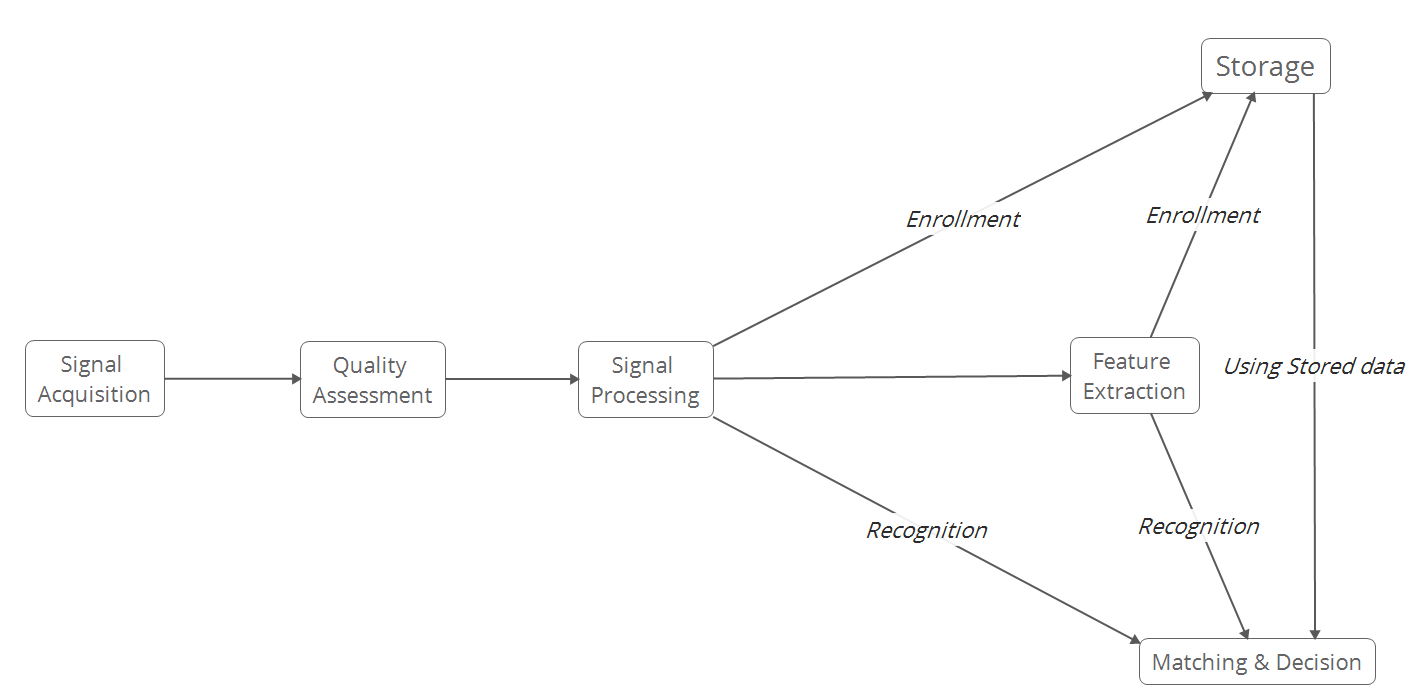
\includegraphics[width = .8\textwidth]{common_bio_process.png}
\caption{The common process for biometric system}
\label{fig:common_process}
\end{figure}

\subsection{Medical Biometrics}
Recently, medical biometrics, a new set of biometric signal are coming to forward( \autocite{Abo:2014biometric}, \autocite{Agrafioti:2012secure}, \autocite{Akhter:2016heart}, cited in  \autocite{Pinto:2018evolution}). In general, medical biometrics depend on physiological characteristics, such as blood pressure, electrocardiogram (ECG), electroencephalogram (EEG), photoplethysmogram (PPG), etc. \autocite{Agrafioti:2011medical}. Pinto et al compared biometric trails, which shows in Table \ref{tab:comparision}.

\begin{table}

\centering
 \begin{tabular}{c c c} 
 Trait & Benefits & Drawbacks \\ [0.5ex] 
 \hline\hline
  & Universality & Requires contact \\ Electrocardiogram(ECG) & Hidden nature & Variability over time \\ & Simple acquisition & \\ 
 \hline
  & Universality & Expensive equipment \\ Electroencephalogram(EEG) & Hidden nature & Vulnerability to noise \\ &  & Variability over time \\ 
 \hline
  & Easily measurable & Easy circumvention \\ Face & Affordable equipment & Depends on face \\ & & Visibility and lighting \\ 
 \hline
  Fingerprint & High performance & Requires contact \\ & permanent over time & \\
 \hline
  Gait & Easy to measure & Low performance \\ & Affordable equipment & Variability over time \\
  \hline
  Iris & High performance & Expensive equipment \\
  \hline
  Palmprint & High measurability & Requires contact \\ & Permanent over time &  \\ 
  \hline
  & Easy to acquire & Low performance \\ Photoplethysmogram(PPG) & Hidden nature & Variability over time \\ & Affordable equipment & \\ 
  \hline
 Voice & Affordable equipment & Low performance \\ [1ex] 
 \hline
\end{tabular}
\caption{Comparison among biometric traits \autocite{Pinto:2018evolution}}
\label{tab:comparision}
\end{table}

Among those biometric traits, the ECG is the most promising signal for biometrics system \autocite{Pinto:2018evolution}. And some researcher thought ECG is difficult to be falsified and can be used for liveness detection as it is a live indicator \autocite{Wang:2007analysis}, but it is not true because of some attack has already be introduced \autocite{Eberz:2017broken,Karimian:2017vulnerability}. 

\subsection{Electrocardiogram}
The ECG signal describes the electrical activity of the heart over time. It is one of the most popular signals for human health. To record an electrocardiogram, the sensor should have at least two metal electrodes that must be in direct contact with the skin\autocite {Blasco:2018feasibility}.

\begin{figure}[H]
\centering
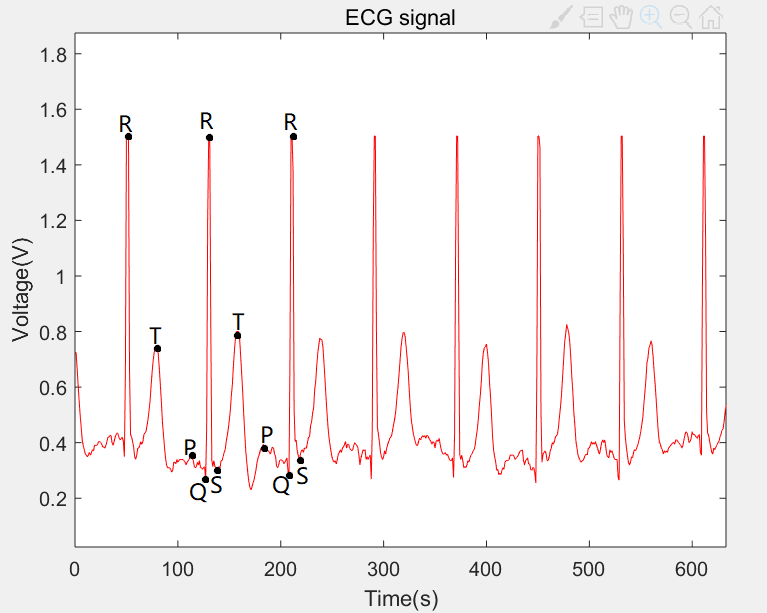
\includegraphics[width = .8\textwidth]{ecg.PNG}
\caption{ECG signals from BIDMC PPG and Respiration Dataset \autocite{PhysioNet}}
\label{fig:ecg}
\end{figure}

Biel et al. \autocite{Biel:2001ecg} are one of the earliest articles which introduce the possibility of using ECG for human identification. Fig \ref{fig:ecg} shows the main components which are used to identify humans include P wave, QRS complex and T wave. The P wave starts for the ECG signal, it represents the depolarization of the right and left atria \autocite{Agrafioti:2011heart}. The QRS wave is the largest wave, describes the depolarization of the ventricles \autocite{Wiki:ecg}. Finally, T wave is the end of a single ECG beat, which shows the repolarization of the ventricles \autocite{Lilly:2012pathophysiology}. For the ECG identification system, there are two main types: fiducial or non-fiducial \autocite{Agrafioti:2012secure}. In fiducial type, the peak of the R wave, T wave and P wave; the R-R interval, R-T interval are considered as features \autocite{Odinaka:2012analysis}. The non-fiducial based method does not use features. Instead, some coefficients will be calculated as a wavelet transform is used in Chan et al.  \autocite{Chan2008wavelet}.

\subsection{Photoplethysmography}
Photoplethysmography (PPG) is a simple technique to detect blood volume changes at skin \autocite{Karimian:2017human}. PPG is widely used in fitness trackers and smart-watches to monitor user's fitness behavior and health statement. The sensors detect the light variations when blood passes through the skin \autocite{Blasco:2018feasibility}. PPG can be gathered from transmissive mode at the fingertip or reflection mode as on the forehead \autocite{wiki:ppg}. Transmissive mode requires the photosensor and LED light to be placed on opposite sides of the finger, so that when blood pass by under the skin, the sensor can detect the difference. For the reflection mode, the sensor and the LED light are deployed on the same side, and the light is reflected into the detector as the blood passes, which is usually used by the wearable device. A common PPG is shown in Fig

\begin{figure}[H]
\centering
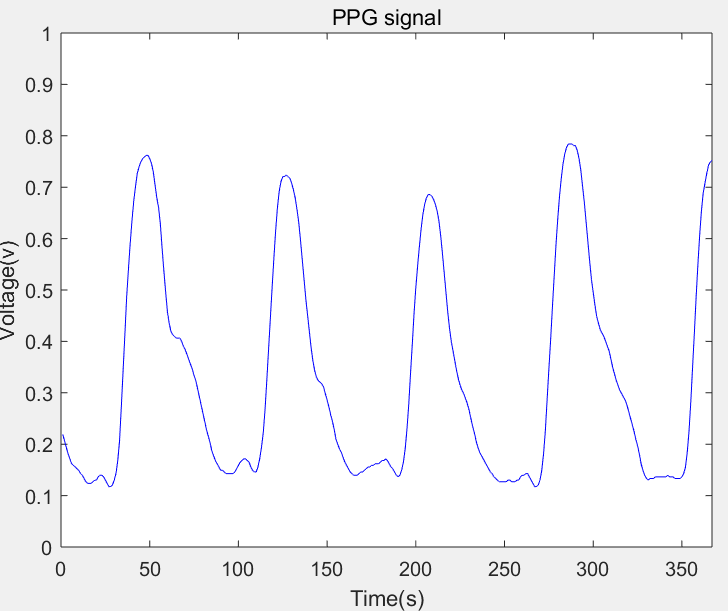
\includegraphics[width = .8\textwidth]{ppg.PNG}
\caption{PPG signals from BIDMC PPG and Respiration Dataset \autocite{PhysioNet}}
\label{fig:ppg}
\end{figure}

\subsection{Devices}
Nowadays, wearable devices become more and more powerful, many of them can trick a person's fitness record by using PPG, a part of which can also read ECG data as a supplement. Table \ref{tab: devices} shows several devices which are used in the commercial area.

\begin{table}[H]
    \centering
    \begin{tabular}{c|c|c}
        Devices & Sensor & Signal  \\
        \hline
        Apple Watch 2015 \autocite{applewatch:edition} & PPG & Light
         \\
         \hline
        Apple Watch Series 4 \autocite{applewatch:series4health&ecg_2019} & PPG & Light
         \\
         & ECG & Electrical
         \\
         \hline
        Nymi Band 2015 & ECG & Electrical
         \\
         \hline
        LG HRM Earphones 2014 & PPG & Light
         \\
         \hline
        JBL Under Armour Sport Wireless Heart Rate \autocite{underarmoursportwirelessheartrate} & PPG & Light
         \\
         \hline
        CardioLeaf FIT & ECG & Electrical
         \\
         \hline
        Fitbit charge3 \autocite{fitbit:charge} & PPG & Light
    \end{tabular}
    \caption{Wearable devices with PPG or ECG sensor,  based on the work by Blasco J et al. \autocite{Blasco:2016survey} }
    \label{tab:devices}
\end{table}

\subsection{Motivation}
Although those attacks on ECG are novel, the effect is limited because they assume the ECG signal of a victim has already captured \autocite{Blasco:2018feasibility}. Simultaneously, PPG is widely used in wearable devices and much easier collect than ECG, especially when a remote PPG collection method is introduced by Verkruysse et al. which can collect PPG remotely (> 1m) with ambient light by inexpensive digital cameras (< \$200) \autocite{Verkruysse2008remotePPG}. Also, since ECG and PPG both represent the activity of the heart and the synchronized ECG and PPG signals are shown in Fig \ref{fig:ppg_ecg}, we thought there might be some correlations between PPG and ECG. Thus, we decided to find a transfer formula by using the neural network to generate ECG against ECG identification system from the collected PPG.

\begin{figure}[H]
\centering
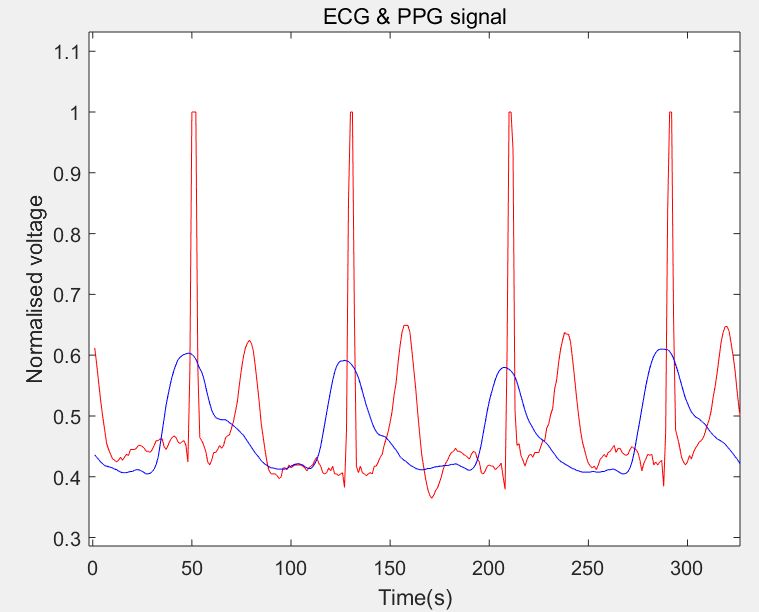
\includegraphics[width = .8\textwidth]{ecg_ppg.PNG}
\caption{Synchronized ECG and PPG signals from BIDMC PPG and Respiration Dataset \autocite{PhysioNet}}
\label{fig:ppg_ecg}
\end{figure}

\section{Machine Learning}
Machine learning is a powerful tool when identifying individuals. For the ECG identification system, there are seven groups classifier to identify individuals:
\begin{enumerate}
    \item kNN classifier
    \item Nearest Center classifier
    \item LDA classifier
    \item Neural network classifier
    \item Generative classifier
    \item Match score classifier
    \item SVM classifier
\end{enumerate}
The SVM classifier is popular and based on machine learning, we will discuss more in this section. Also, the neural network is another widely used machine learning method in a biometric identification system. Because we will estimation a transfer function from PPG to ECG by the neural network, it will also be introduced.

\subsection{SVM}
Support vector machines(SVM) is considered as a discriminant classifier which defined by a separation hyperplane \autocite{patel_2019}. It is a supervised learning model which means the training sample should be labeled manually at first to let the machine learn the rule for distinguishing or analyzing data. SVM is used in classifying text and hypertext, images, Hand-written, and biological \autocite{wiki:svm}. To classify data, the machine should determine the incoming data belong to which class. In SVM, the data point is viewed as p-dimension vector, and if there is a (p-1) dimension hyperplane which can separate vectors, it is called linear classifier. A maximum-margin classifier is shown in Fig \ref{fig:svm_liner}, the blue and green point is a data point, the hyperplane is the red line in the middle. Because of the distance from hyperplane to the nearest data on each class is maximized, it is a maximum margin classifier, and the stability of the classifier is optimal. Otherwise, if the classifier is not maximum - margin mode, the hyperplane will be closer to one class, when a new data point comes in, the possibility of judge the new point as the class which has more distance to the hyperplane than the other might increase, that is not an optimal situation.

\begin{figure}[H]
\centering
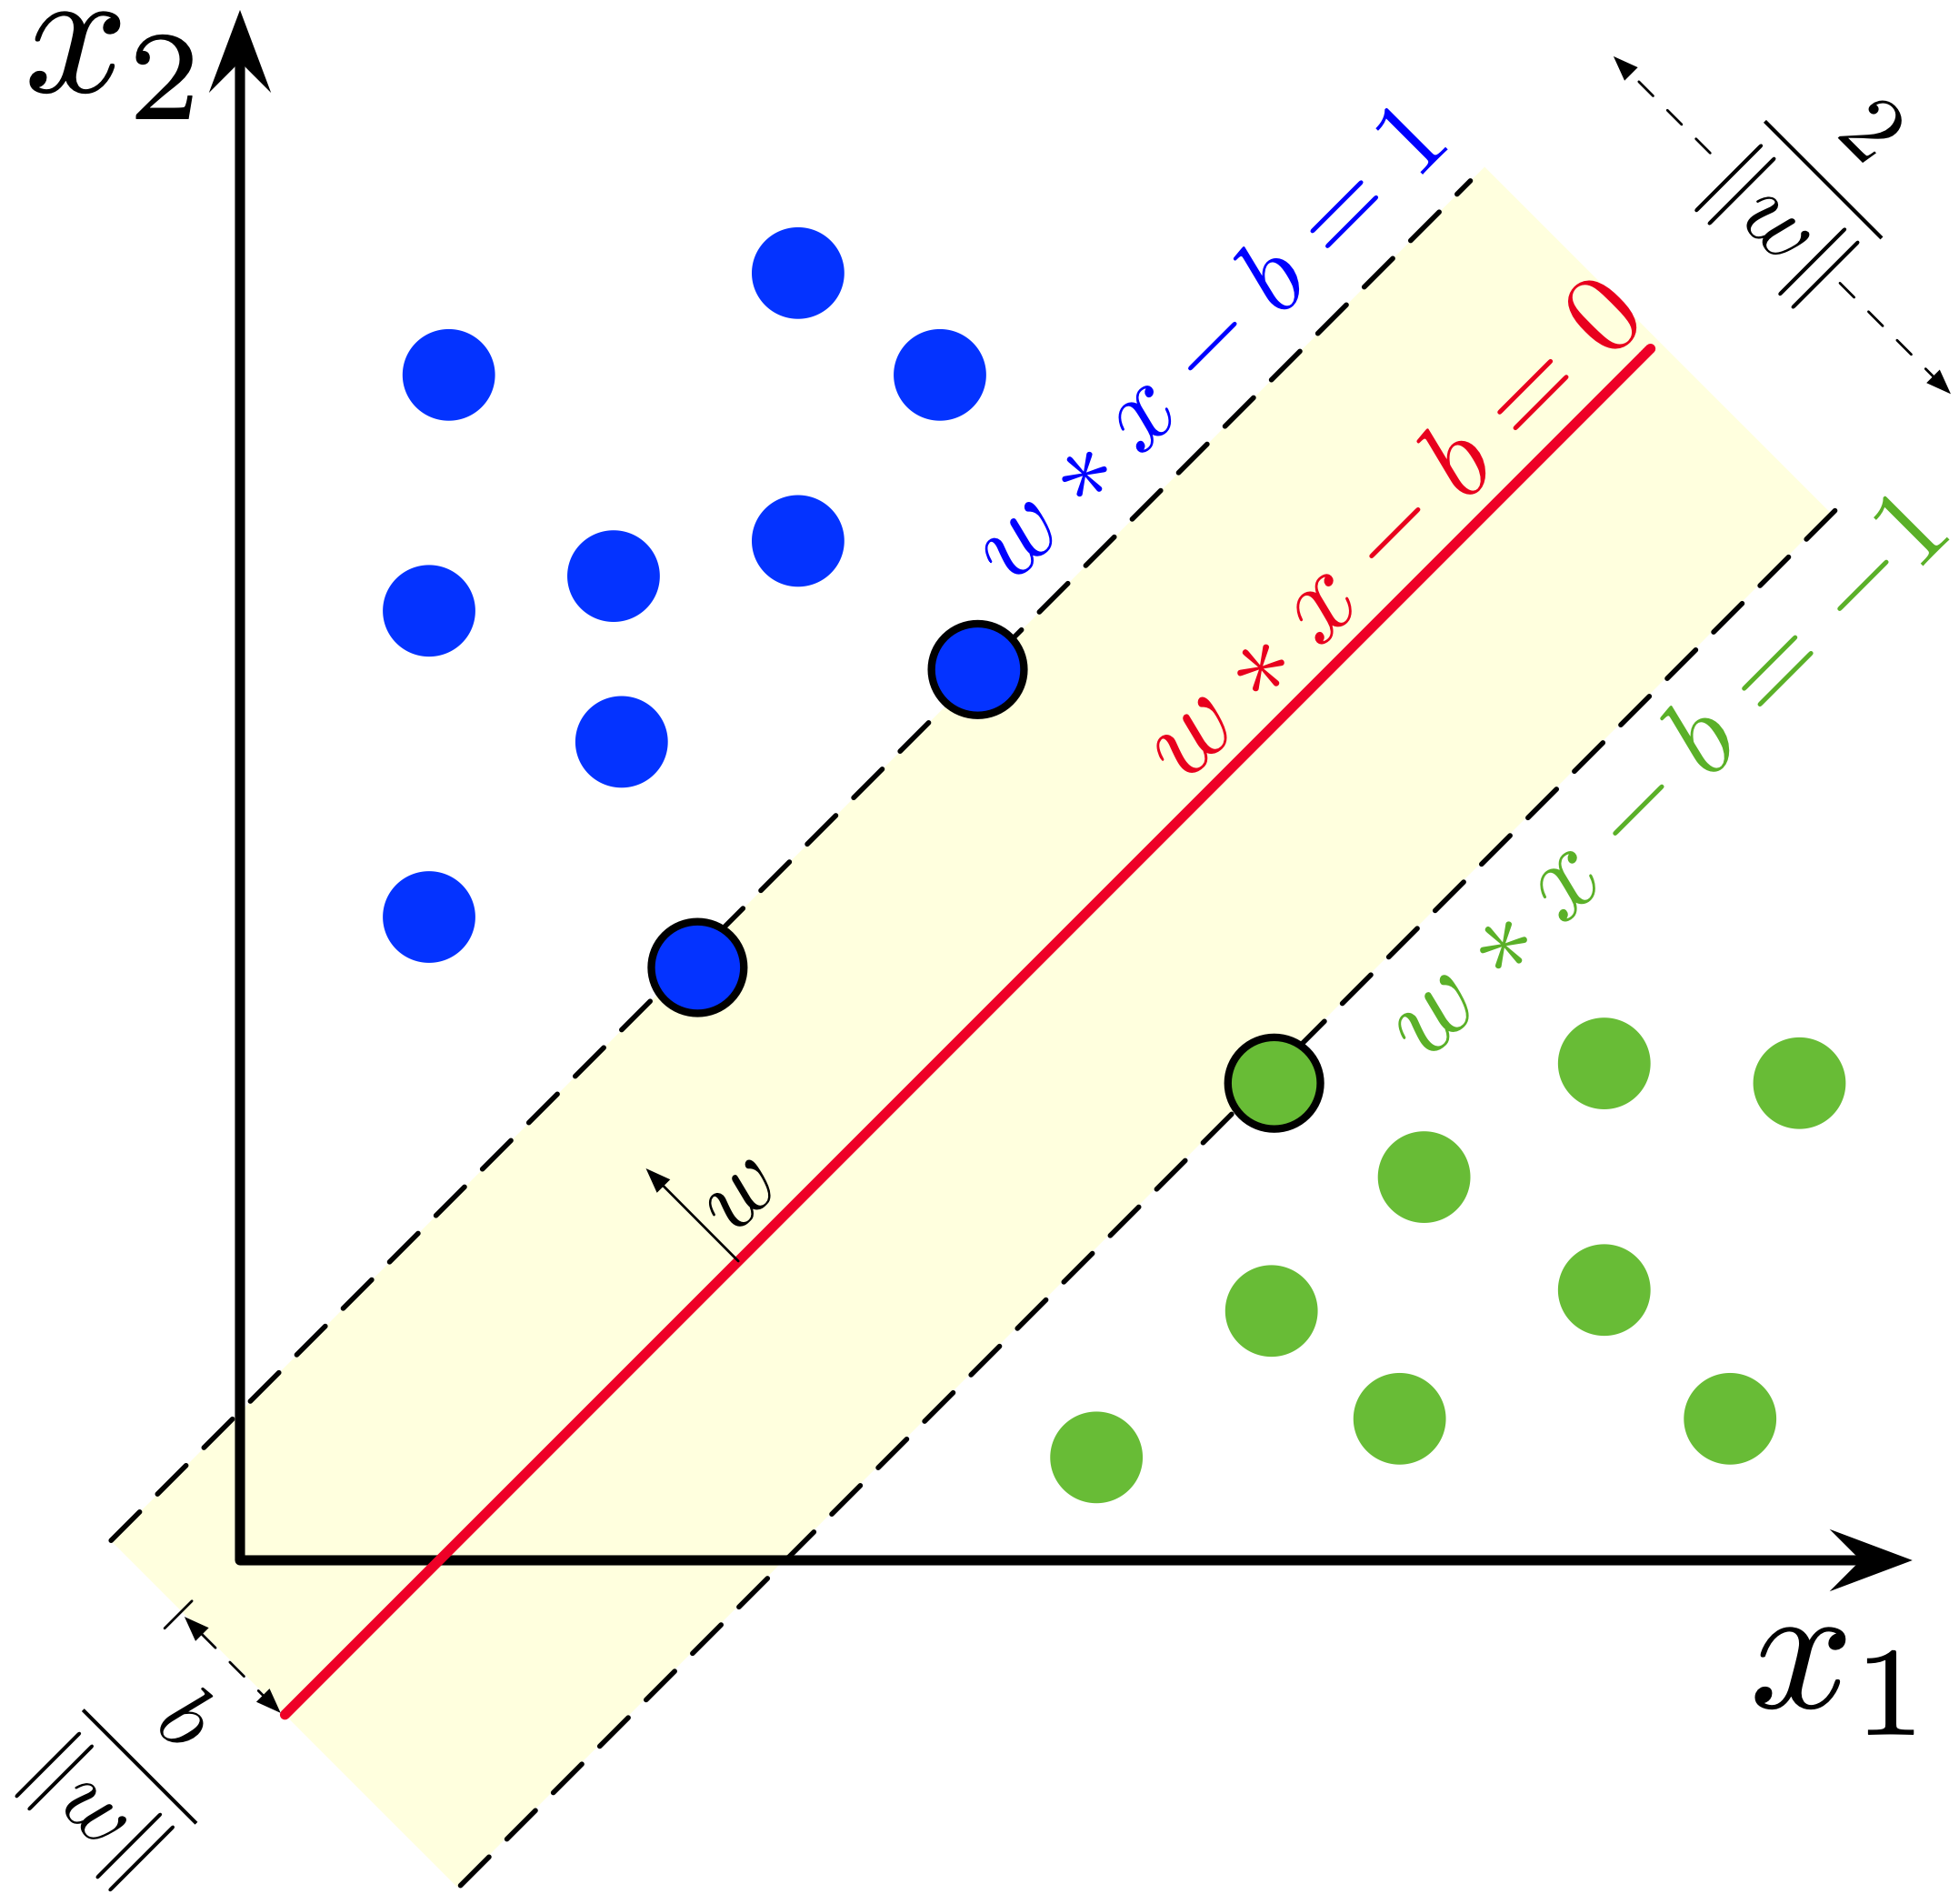
\includegraphics[width = .8\textwidth]{SVM_margin.png}
\caption{Maximum-margin hyperplane \autocite{wiki:svm}}
\label{fig:svm_liner}
\end{figure}

However, the sets to discriminate are not often able to be separated by a linear method in that space \autocite{wiki:svm}. An example dataset is shown at Fig \ref{Fig.sub.1}. It is obviously, the linear classifier cannot separate by a hyperplane in a one dimension line (consider the situation is in two dimensions). In this situation, there is a transfer called kernel which transfers the dataset to higher dimension, separate dataset by a hyperplane and transfers the hyperplane back to origin dimension. As the graph Fig \ref{Fig.sub.2}, Fig \ref{Fig.sub.3} shows, a kernel function \[w = x^2 + y ^2\] is used to transfer so that the hyperplane in Y-Z axes is found and the hyperplane is shown as the circle in X-Y axes which is the origin dimension.

\begin{figure}[H]
\centering 
\subfigure[Non-linear dataset, X-Y axises]{
\label{Fig.sub.1}
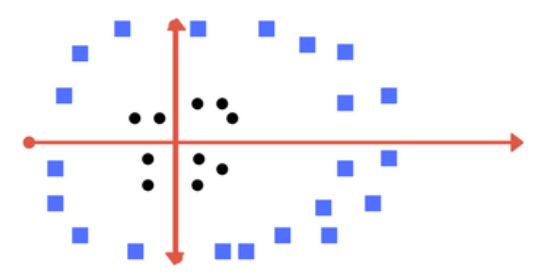
\includegraphics[width=0.3\textwidth, height=0.33\textwidth]{Kernel_Machine1.png}}
\subfigure[Dataset in high dimension, Y-Z axises]{
\label{Fig.sub.2}
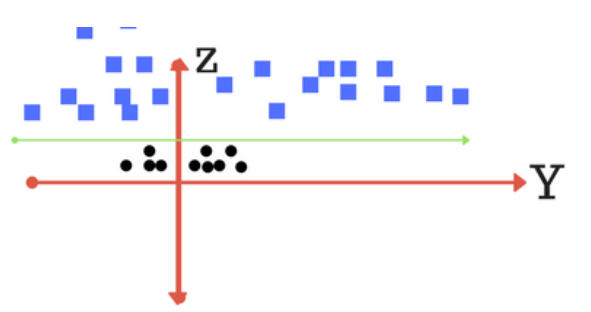
\includegraphics[width=0.3\textwidth, height=0.33\textwidth]{Kernel_Machine2.png}}
\subfigure[Hyperplane at origin dimension, X-Y axises]{
\label{Fig.sub.3}
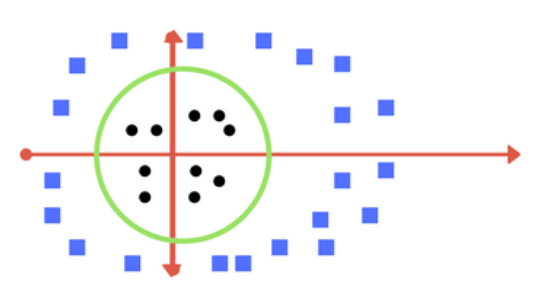
\includegraphics[width=0.3\textwidth, height=0.33\textwidth]{Kernel_Machine3.png}}
\caption{Example for kernel mode SVM \autocite{patel_2019}}
\label{Fig.main}
\end{figure}

SVM belong to a family of generalized linear classifiers,the main drawbacks contain following aspects \autocite{wiki:svm}:
\begin{enumerate}
    \item Needs of the complete label of data to train the model
    \item Uncalibrated class membership probabilities, which avoids estimating probabilities on finite data.
    \item Only suitable for distinguish two class data, any multi-class task should be reduced to two class task. 
    \item The parameters of solved model are difficult to translate.
\end{enumerate}

\subsection{Neural Network}
SVM is not a good choice for estimate ECG. As a classifier, which is the area of expertise for SVM, there is a drawback. The SVM will suffer from dimension curse. For each signal subject, ECG signal will be considered as multiple dimensions. For instance, in Ye's method\autocite{Ye:2012heartbeat}, even reduced the dimension by Principal components analysis(PCA) there are still 26 features for each subject which mean each dimension will influence the decision making, both the efficiency and accuracy will decrease. We consider using a neural network. The basis of a neural network, or neural network, is using networks of functions to understands and translate input data to the expected output data. The concept of a neural network was inspired by the neurons in the human brain. A neural network is a tool used in a machine learning algorithm but not the algorithm, and it is a piece in a machine learning algorithm to process complex input data \autocite{Build_with_ai:deepai_2019}. 

Many problems are using the neural network today, include spam email filtering, recognition for speech and image. For instance, in image recognition, the neural network learns to identify images that contain cats without any prior knowledge about cats but analyzing images that have been labeled manually as 'cat' or 'no cat' \autocite{wiki:neuralnetwork}. The neural network has become more and more popular in the prediction area as well. For example, a deep neural network has an advantage in prediction the activity of potential drug molecules compares with other machine learning method \autocite{Ma:2015deep}. Also, the neural network was used to predict the effects of defects in RNA splicing \autocite{Xiong:2015human}.

A standard neural network composed of many connected processors. The processors, which are called neurons,  producing real-valued activation, except for input neurons, other neurons get activated through weighted connection from previously active neurons, the input neurons get activated by data input \autocite{Schmidhuber:2015deep}. Feedforward neural network is widely used in many applications, which map fixed-size input to a fixed-size output by layer to layer \autocite{Lecun:2015deep}. To map the input and output, a neurons layer compute a weighted sum of the input from the previous layer and pass the result by a non-layer function, the layers exclude input and output layer are considered as a hidden layer. The function normally is the rectified linear unit(ReLU) which is suitable for a neural network with many layers. 

Simple stochastic gradient descent was used to train the multilayer architectures network. If the input functions and weights are relatively smooth, the gradients can be computed by the backpropagation procedure \autocite{Lecun:2015deep}. The backpropagation algorithm is a key trigger for renewed interest in neural networks \autocite{wiki:neuralnetwork}. In the backpropagation algorithm, weights at each node will be modified to distribute the error back to layers. However, in the late 1990s, the simple gradient descent was commonly considered as a method which could be stuck in poor local minima weight \autocite{Lecun:2015deep}. But in practice, the situation of poor local minima are rarely in large network \autocite{Lecun:2015deep}.

\section{Related Work}
\subsection{Estimate ECG}
Banerjee R et al. introduced a method to estimation ECG features include PR interval, QRS interval, QT interval by PPG \autocite{Banerjee:2013estimation}. The author wants to find a feasible and cheap method to provide a basic screening system which can make an alert for possible unwellness toward to those people who are suffering from heart diseases or prone to heart attack. Therefore, they were trying to use PPG, which is a cheap, non-invasive and widely used signal, to estimation the range of some parameters of great value in ECG signal which are PR, RR, QRS, and QT interval. 

\begin{figure}[H]
\centering
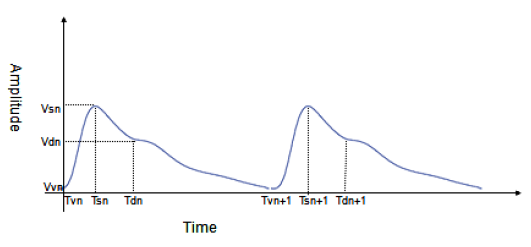
\includegraphics[width = .8\textwidth]{ppg1.PNG}
\caption{PPG feature extraction \autocite{Banerjee:2013estimation}}
\label{fig:ppg1}
\end{figure}

The Fig \ref{fig:ppg1} shows labeled PPG signal. The author first extracts ten dimension features from PPG which will be described below by the labels in the picture:

\[\textrm{1. Peak to Peak Interval: }T_{pp} = T_{{s_n}+1} - T_{s_n}\]
\[\textrm{2. Pulse Interval: }T_{pi} = T_{{v_n}+1} - T_{v_n}\]
\[\textrm{3. Pulse Height: }V_{ph} = V_{s_n} - V_{v_n}\]
\[\textrm{4. Crest Time: }T_{cr} = T_{s_n} - T_{v_n}\]
\[\textrm{5. Delta Time: }T_{del} = T_{d_n} - T_{s_n}\]
\[\textrm{6. Dict. Time: }T_{dic} = T_{d_n} - T_{v_n}\]
\[\textrm{7. Falling Time: }T_{f} = T_{{v_n}+1} - T_{s_n}\]
\[\textrm{8. Dic2Min Time: }T_{dm} = T_{{v_n}+1} - T_{d_n}\]
\[\textrm{9. Rising Slope: }S_{r} = \frac{V_{s_n} - V_{v_n}}{T_{s_n} - T_{v_n}}\]
\[\textrm{10. Falling Slope: }S_{f} = \frac{V_{{v_n} + 1} - V_{s_n}}{T_{{v_n} + 1} - T_{s_n}}\]

Machine learning methods will be affected by dimensional disasters because as the dimension increases, the data will quickly become sparse, which means that if some input data is less relevant to the target, as the data dimension increases, the machine's Learning performance will be reduced. Therefore, the author selects features by using the maximum information coefficient (MIC) and Pearson product moment correlation coefficients to find the relationship between ECG and PPG features. The author found the relation between the ECG parameter and PPG features as follows:
\[F_{PR} = \{f^1, f^2, f^3, f^4, f^6, f^9, f^{10}\}\]
\[F_{RR} = \{f^1, f^2, f^6, f^7\}\]
\[F_{QRS} = \{f^4, f^5, f^6, f^{10}\}\]
\[F_{QT} = \{f^1, f^2, f^5, f^6, f^7, f^{10}\}\]

The author train different ECG classifier by the selected PPG features and the accuracy they got is in table \ref{tab:perfoemance_ppges}:

\begin{table}[H]
    \centering
    \begin{tabular}{c|c|c}
         ECG param& with ANN(\%) & with SVm(\%) \\
    \hline
         PR & 88.5 & 90.3 \\
         RR & 93.9 & 94.6 \\
         QRS & 84.1 & 84.9 \\
         QT & 91.1 & 92.6 
    \end{tabular}
    \caption{Performance of using selected features \autocite{Banerjee:2013estimation}}
    \label{tab:perfoemance_ppges}
\end{table}

\subsection{Current Attacks}
As mentioned before, the biometric identification system does solve some problems in the traditional identification system, such as lost or forgotten because they are based on physical objects or the user's knowledge. However, nothing is perfect; biometrics leads to some brand-new risks. Fingerprint and face recognition are most common identification method; both can be easily observed and replicated by attacker \autocite{Eberz:2018your}. For example, fingerprints can be collected from nearly everywhere such as the office door and a used cup. Moreover, the face identification system might suffer the attack by using a 2-D photo. The photo of the victim can be grab from social media(Facebook), personal blog or CV of the victim.

Medical biometrics has become a favorite research subject. In 2010, Odinaka et al. thought ECG are challenging to forge \autocite{Odinaka:2010ecg}. Agrafioti et al. mentioned the main strength of medical biometrics is robustness to reply, obfuscation and circumvention attack in 2011 \autocite{Agrafioti:2011heart}.

However, even existing ECG biometrics are considered offering a high-security level against impersonation attacks \autocite{Blasco:2018feasibility}, it is not perfect, some attack has already been introduced. For instance, Eberz et al. present a presentation attack against ECG biometrics in Nymi band by transfer attacker's ECG to victim's ECG and reply the transferred ECG signals \autocite{Eberz:2017broken}. In the remainder of this section, we will discuss current attacks for both traditional biometrics and medical biometric.

\subsubsection{Attacks on traditional biometrics}
For traditional biometrics, the most common signals used to identify human is the face, fingerprint, and iris as static features, the voice is widely used to distinguish human as a dynamic signal when people make a phone call. However, because of the popularity of that method is so high that some high performance with low-cost attacks has already existed.

In 2012, Galbally J et al.  \autocite{Galbally:2012iriscode} introduced an attack which is based on iris code to rebuild origin iris information. The experimental result showed that the reconstructed images are very realistic and might have a chance to break through the iris identification system. As a result, the possibility of unauthorized access is 75\% to 94\%.

In 2015, Ergünay S K et al.  \autocite{Ergunay:2015voicevulnerability} introduced a voice spoofing data-set which include threat contain reply, speech synthesis, and voice conversion. Also, an experimental were provided to show the effect of an automatic speaker verification system. The spoofing false acceptance rate is 96.5\% for Male and 81.5\% on Female.

In 2017, Chen et al.  \autocite{Chen:2017spoofing}researched a method to spoofing faces by using makeup. They found automated face recognition machine are suffered from makeup attack. They thought it is easy for the malicious individual to trick identification system by using makeup. However, the worst case for identification in their research is around 50\% when testing 30 probe image with commercial Off-The-Shelf face software.

\subsubsection{Attacks on medical biometrics}
Traditional biometric features are suffered from forge attack, but the medical biometric features like ECG are not easy to counterfeit because of the uniqueness of the signal for the individual. However, since 2003 the dynamical method for generating ECG was provided by McSharry P E et al.  \autocite{Mcsharry:2003dynamical} the forge attack to ECG became possible. In their research, the operator can specify the mean and deviation of the heart rate, the power of R and the shape of the PQRST cycle. The attacker might generate a realistic ECG signal to access the ECG identification system.

Moreover, In 2017, Eberz et al.  \autocite{Eberz:2017broken} provided an attack target on ECG biometric identification system. They demonstrate the attack which is based on the Nymi band which is a wrist band as a biometric identification system. The attack is based on a mapping function which is trained by previously collected ECG signals and replay the manufactured ECG to pass the authentication by Nymi band. The result of the attack, 81\% success rate for the best case which used the signal collected from Nymi band, for remaining signal sources like the signal received from medical ECG monitor, the success rate is 62\%. In the same year, Karimian N, Woodard D L, and Forte D introduced another presentation attack \autocite{Karimian:2017vulnerability} which map the attacker's ECG to victim's by using captured victim's ECG. The mapping function is suitable for both off-line attack and online attack which the attacker has less time and resources. For the experiment result, the average success rate is 97.43\% and 94.17\% towards non-fiducial and fiducial based ECG identification system respectively. In the online mode, the performance decreased for 5.65\% in the non-fiducial system but unaffected on the fiducial system.

\section{Conclusion}

\printbibliography

\end{document}
